%!TEX TS-program = xelatex
%!TEX encoding = UTF-8 Unicode

En este ejercicio buscaremos una definición de roles de nodes dentro de las comunicades para así conocer aquellos que cambian de una comunidad a otra, cambian de rol dentro de la misma comunidad e incluso ubicar aquellos que contribuyen de manera positiva a mantener una buena comunicación entre distintas comunidades.
A cada nodo podemos asignarle un rol dentro de la red dependiendo de su conectividad dentro del módulo al que pertenece y su conectividad con el resto de las comunidades, luego de definir la estructura modular de la red (realizado mediante el algoritmo de Louvain). 
Comparamos la media de cantidad de nodos de cada rol en cada estadío del sueño contra el estadío ‘despierto’, para cada valor de densidad. Se hace una comparación estadística en la cual se observan muy pocas diferencias significativas.


\subsubsection{Connector Nodes}
La cantidad de Connector Nodes crece con el incremento de la densidad para todos los estadíos del sueño y para el estado despierto. No se hallaron diferencias significativas aunque para todos los casos los estadíos de sueño se observaron valores ligeramente más elevados que el estado despierto.


\begin{figure}[H]
    \centering
    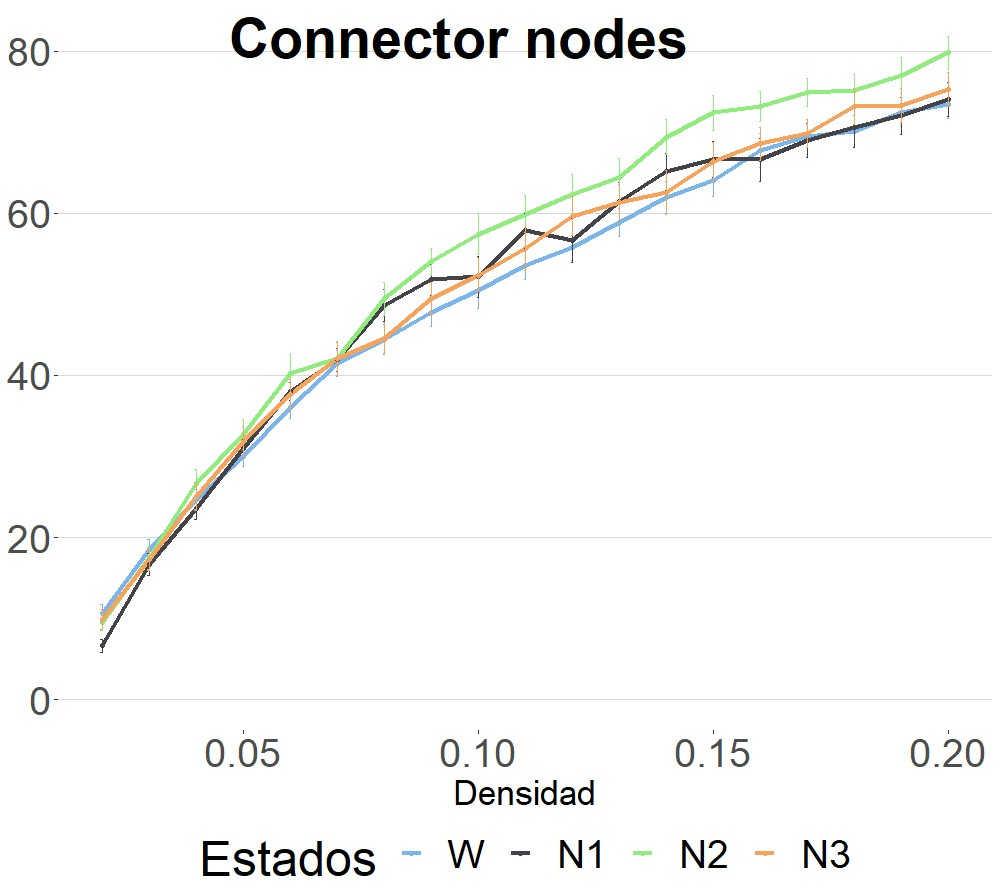
\includegraphics[width = 5in]{img/5_connectornodes.jpg}
    \caption{Connector Nodes}
    \label{fig:5_connectornodes}
\end{figure}

\subsubsection{Hubs}
La diferencia entre el estado despierto y las distintas etapas del sueño no resulta significativa en ningún caso. Puede observarse como la cantidad de hubs se incrementa a medida que se incrementa la densidad. El comportamiento resulta más similar entre W y N1 y N2 ya que muchas veces se cruzan sus trazas. El gráfico de W versus N3 presenta la mayor diferencia ya que la traza de N3 se encuentra siempre por encima de la de W.

\begin{figure}[H]
    \centering
    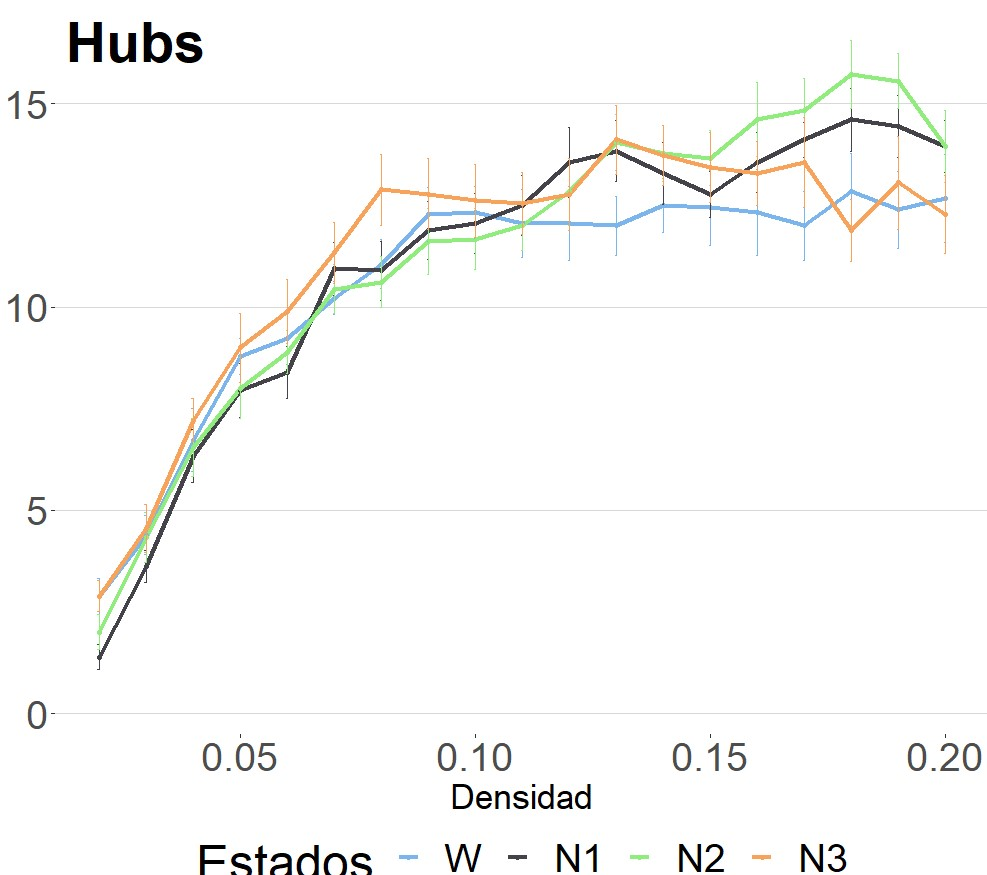
\includegraphics[width = 5in]{img/5_hubs.jpg}
    \caption{Hubs}
    \label{fig:5_hubs}
\end{figure}

\subsubsection{Provincial Hubs}
La cantidad de Provincial Hubs decrece con el incremento de la densidad para todos los estadíos del sueño y
para el estado despierto. Vemos que N1 se mantiene por encima de W en la mayoría de los puntos y N3 por debajo.

\begin{figure}[H]
    \centering
    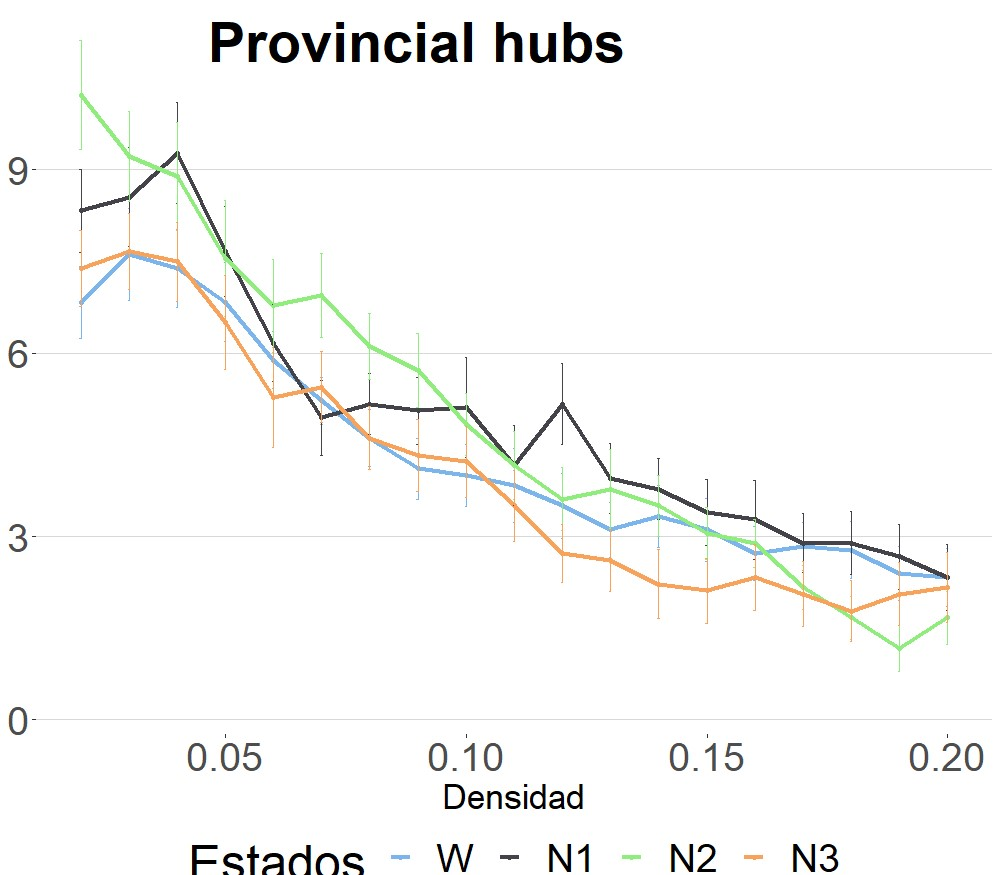
\includegraphics[width = 5in]{img/5_provincialhubs.jpg}
    \caption{Provincial Hubs}
    \label{fig:5_provincialhubs}
\end{figure}


\subsubsection{Provincial Nodes}
La cantidad de Provincial Nodes decrece con el incremento de la densidad para todos los estadíos del sueño y para el estado despierto. Se hallaron diferencias significativas para dos valores de baja densidad del comparativo de W con N1
y en un caso de baja densidad del comparativo de W con N2. En los dos puntos significativos el estadío de sueño presentó un número mayor de PN para ese valor de densidad. En los tres comparativos se observó el mismo comportamiento: el estadío del sueño comienza tomando valores superiores a W para bajas densidades y, a medida que se incrementa la densidad, a partir de 0.08 aproximadamente se invierte el orden y W toma valores más elevados que los estadíos del sueño.


\begin{figure}[H]
    \centering
    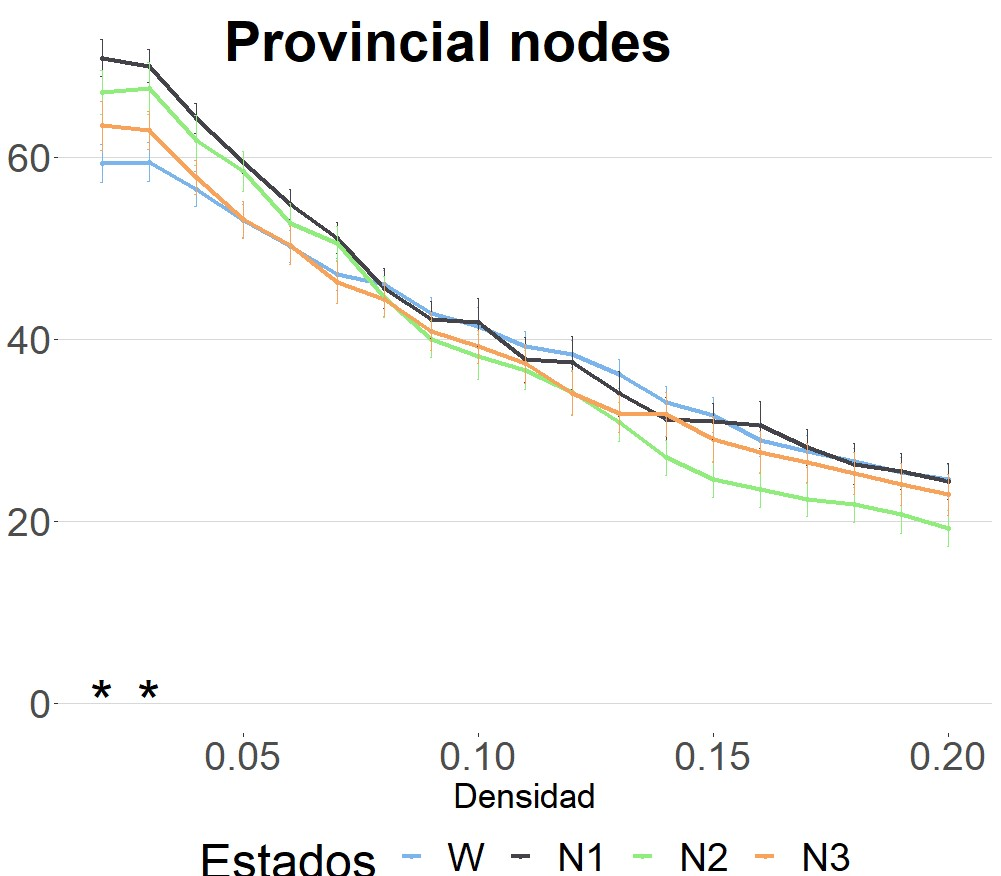
\includegraphics[width = 5in]{img/5_provincialnodes.jpg}
    \caption{Provincial Nodes}
    \label{fig:5_provincialnodes}
\end{figure}


\subsubsection{Visualizar para densidad 0.08}
A continuación fijando una densidad de 0.08, se hace una visualización de la red promedio binaria para cada estadío, discriminando los nodos según su rol. Se definió este nivel de densidad, ya que se probaron con varios, pero  para obtener una lectura más clara de las conexiones $0.08$ fue el que mejor resultado nos dio ya que a medida que se aumentaba la densidad las conexiones se hacían más complejas de describir, algo que notamos fue mayor cambio a central nodes en la región parietal.

\begin{figure}[H]
    \centering
    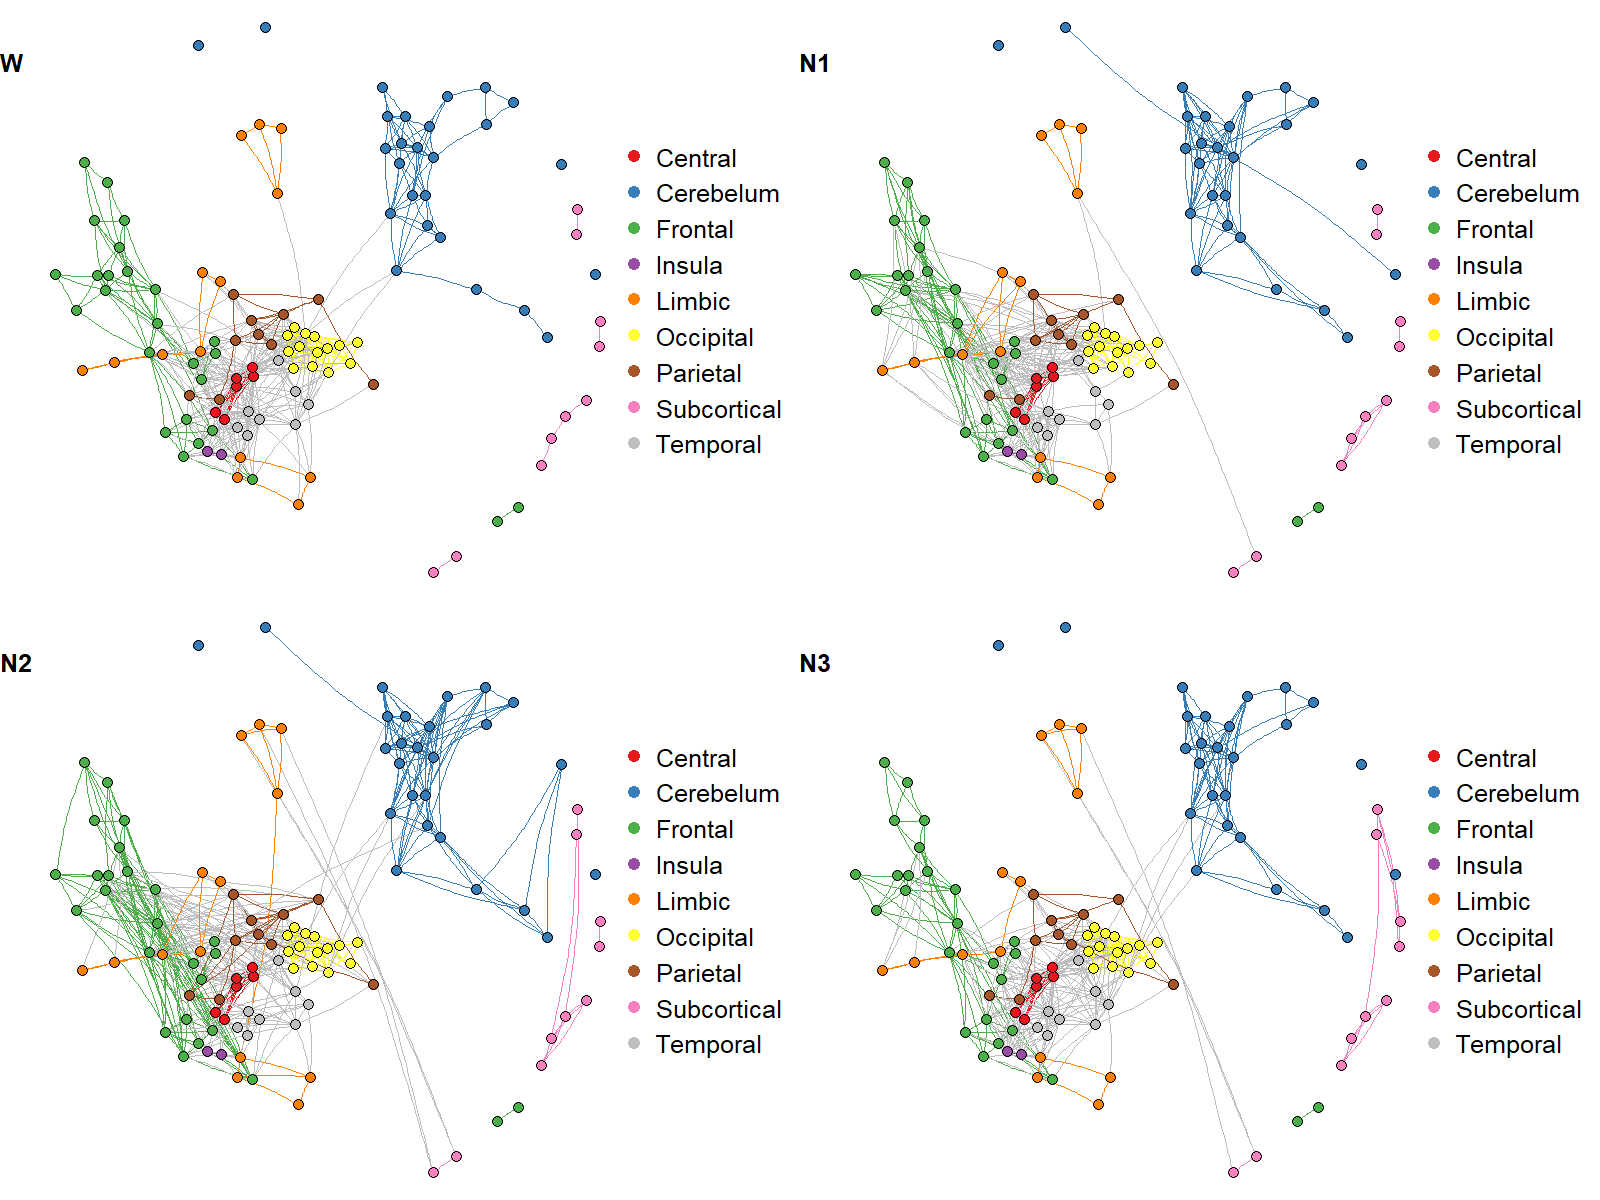
\includegraphics[width=\textwidth]{img/5_redescerebro_008.png}
    \caption{Zonas del Cerebro}
    \label{fig:Ejer5_redescerebro_008}
\end{figure}

\begin{figure}[H]
    \centering
    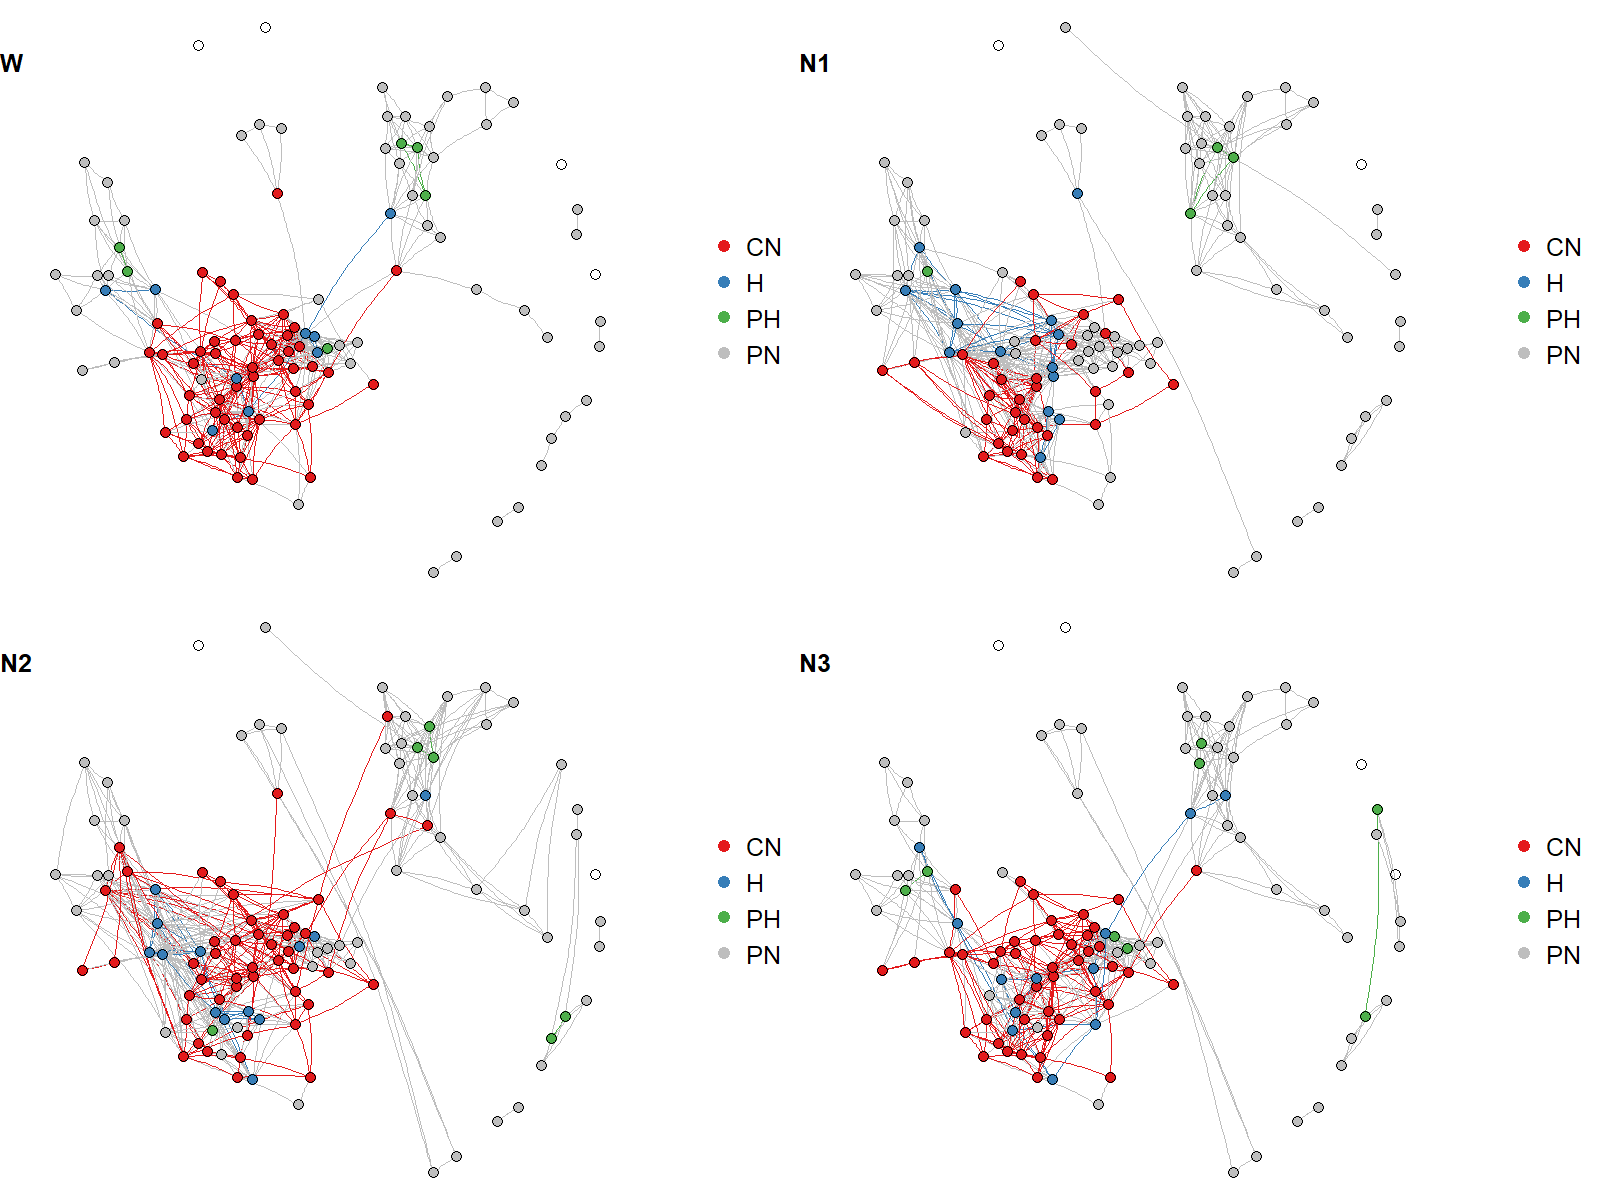
\includegraphics[width=\textwidth]{img/5_redes_roles008.png}
    \caption{Roles con Densidad 0.08}
    \label{fig:Ejer5_redes_roles008}
\end{figure}

No observamos claramente la relación entre agrupamientos funcionales y anatómicos sin embargo podemos concluir lo siguiente:

\begin{itemize} 
\item Para todos los estadíos del sueño la región (anatómica) Subcortical corresponde con Provincial Nodes (PN).
\item Para todos los estadíos del sueño casi toda la región (anatómica) Cerebelum corresponde con PN, aunque presenta algunos Hubs (H) y Provincial Hubs (PH)
\item La región anatómica Insula varía su comportamiento en cada estadío del sueño. Para los estados N1 y N2 se compone únicamente de Central Nodes (CN), en el estadío N3 de H y en el W de PN.
\item No observamos ningún patrón relevante para el resto de las regiones del cerebro debido a  que presentan varios tipos distintos de nodos en todos los estadíos y los mismos sufren modificaciones sin un patrón claro.
\end{itemize}